\documentclass[a4paper,12pt]{article}
%\documentclass[a4paper,10pt]{scrartcl}

\usepackage[utf8x]{inputenc}
\usepackage{amsfonts}
\usepackage{amsmath,esint}
\usepackage{graphicx}
\usepackage{pdfpages}
\usepackage{sansmath}
\usepackage{hyperref}
\usepackage{natbib}
\usepackage{caption}
\usepackage{tikz}
\usepackage{algorithm}
\usepackage[noend]{algpseudocode}

\usepackage{titling}
\setlength{\droptitle}{-5em}   % This is your set screw
\renewcommand{\familydefault}{\sfdefault}


% ------------------------------------------------------------------
\newcommand{\permittivity}{\boldsymbol{\varepsilon}}
\newcommand{\conductivity}{\boldsymbol{\sigma}}
\newcommand{\permittivityperturb}{\hat{\boldsymbol{\varepsilon}}}
\newcommand{\conductivityperturb}{\hat{\boldsymbol{\sigma}}}
\newcommand{\permittivitysolu}{\boldsymbol{\varepsilon}_*}
\newcommand{\conductivitysolu}{\boldsymbol{\sigma}_*}
% ------------------------------------------------------------------
\newcommand{\umat}{\mathbf{u}}
\newcommand{\Lw}{\mathbf{L}_w}
\newcommand{\sw}{\mathbf{s}_w}
\newcommand{\dw}{\mathbf{d}_w}
\newcommand{\dwo}{\mathbf{d}^o_w}
\newcommand{\dwos}{\mathbf{d}^{o,s}_w}
\newcommand{\Mw}{\mathbf{M}_w}
\newcommand{\umatdot}{\dot{\mathbf{u}}}
\newcommand{\ew}{\mathbf{e}_w}
\newcommand{\vw}{\mathbf{v}_w}
\newcommand{\gwe}{\mathbf{g}_{\varepsilon}}
\newcommand{\gws}{\mathbf{g}_{w,\sigma}}
\newcommand{\dt}{\Delta t}
\newcommand{\dx}{\Delta x}
\newcommand{\dz}{\Delta z}
\newcommand{\dsigmaw}{\dsigma_w}
\newcommand{\depsi}{\Delta\boldsymbol{\varepsilon}}
\newcommand{\stepepsi}{\alpha_\varepsilon}
\newcommand{\stepsigm}{\alpha_\sigma}
\newcommand{\kappaepsi}{\kappa_\varepsilon}
\newcommand{\kappasigm}{\kappa_{w,\sigma}}
\newcommand{\depsimomentum}{\Delta\boldsymbol{\varepsilon}_\bullet}
% ------------------------------------------------------------------
\newcommand{\electpotential}{\boldsymbol{\varphi}}
\newcommand{\Ldc}{\mathbf{L}_{dc}}
\newcommand{\sdc}{\mathbf{s}_{dc}}
\newcommand{\Sdc}{\mathbf{S}_{dc}}
\newcommand{\ddc}{\mathbf{d}_{dc}}
\newcommand{\ddco}{\mathbf{d}_{dc}^o}
\newcommand{\ddcos}{\mathbf{d}_{dc}^{o,s}}
\newcommand{\Mdc}{\mathbf{M}_{dc}}
\newcommand{\edc}{\mathbf{e}_{dc}}
\newcommand{\vdc}{\mathbf{v}_{dc}}
\newcommand{\gdc}{\mathbf{g}_{dc}}
\newcommand{\dsigmadc}{\dsigma_{dc}}
\newcommand{\stepdc}{\alpha_{dc}}
\newcommand{\dsigmmomentum}{\dsigma_{dc\,\bullet}}
% ------------------------------------------------------------------
\newcommand{\Ewe}{\Theta_{w,\varepsilon}}
\newcommand{\Ewes}{\Theta_{w,\varepsilon}^s}
\newcommand{\Ews}{\Theta_{w,\sigma}}
\newcommand{\Ewss}{\Theta_{w,\sigma}^s}
\newcommand{\Ew}{\Theta_{w}}
\newcommand{\Edcs}{\Edc^s}
\newcommand{\Edc}{\Theta_{dc}}
\newcommand{\dsigma}{\Delta\boldsymbol{\sigma}}
\newcommand{\Ewphase}{\Theta_{w,\phi}}
\newcommand{\Ewenvel}{\Theta_{w,E}}
% ------------------------------------------------------------------

\title{Empirical depth-time parameters of investigation of a GPR experiment}
\author{Diego Domenzain}
\date{}

\begin{document}
\maketitle

% ------------------------------------------------------
%
% ------------------------------------------------------
\section{Common offset two-way time}
%
%
\begin{figure}[!h]
\centering
% left low right up
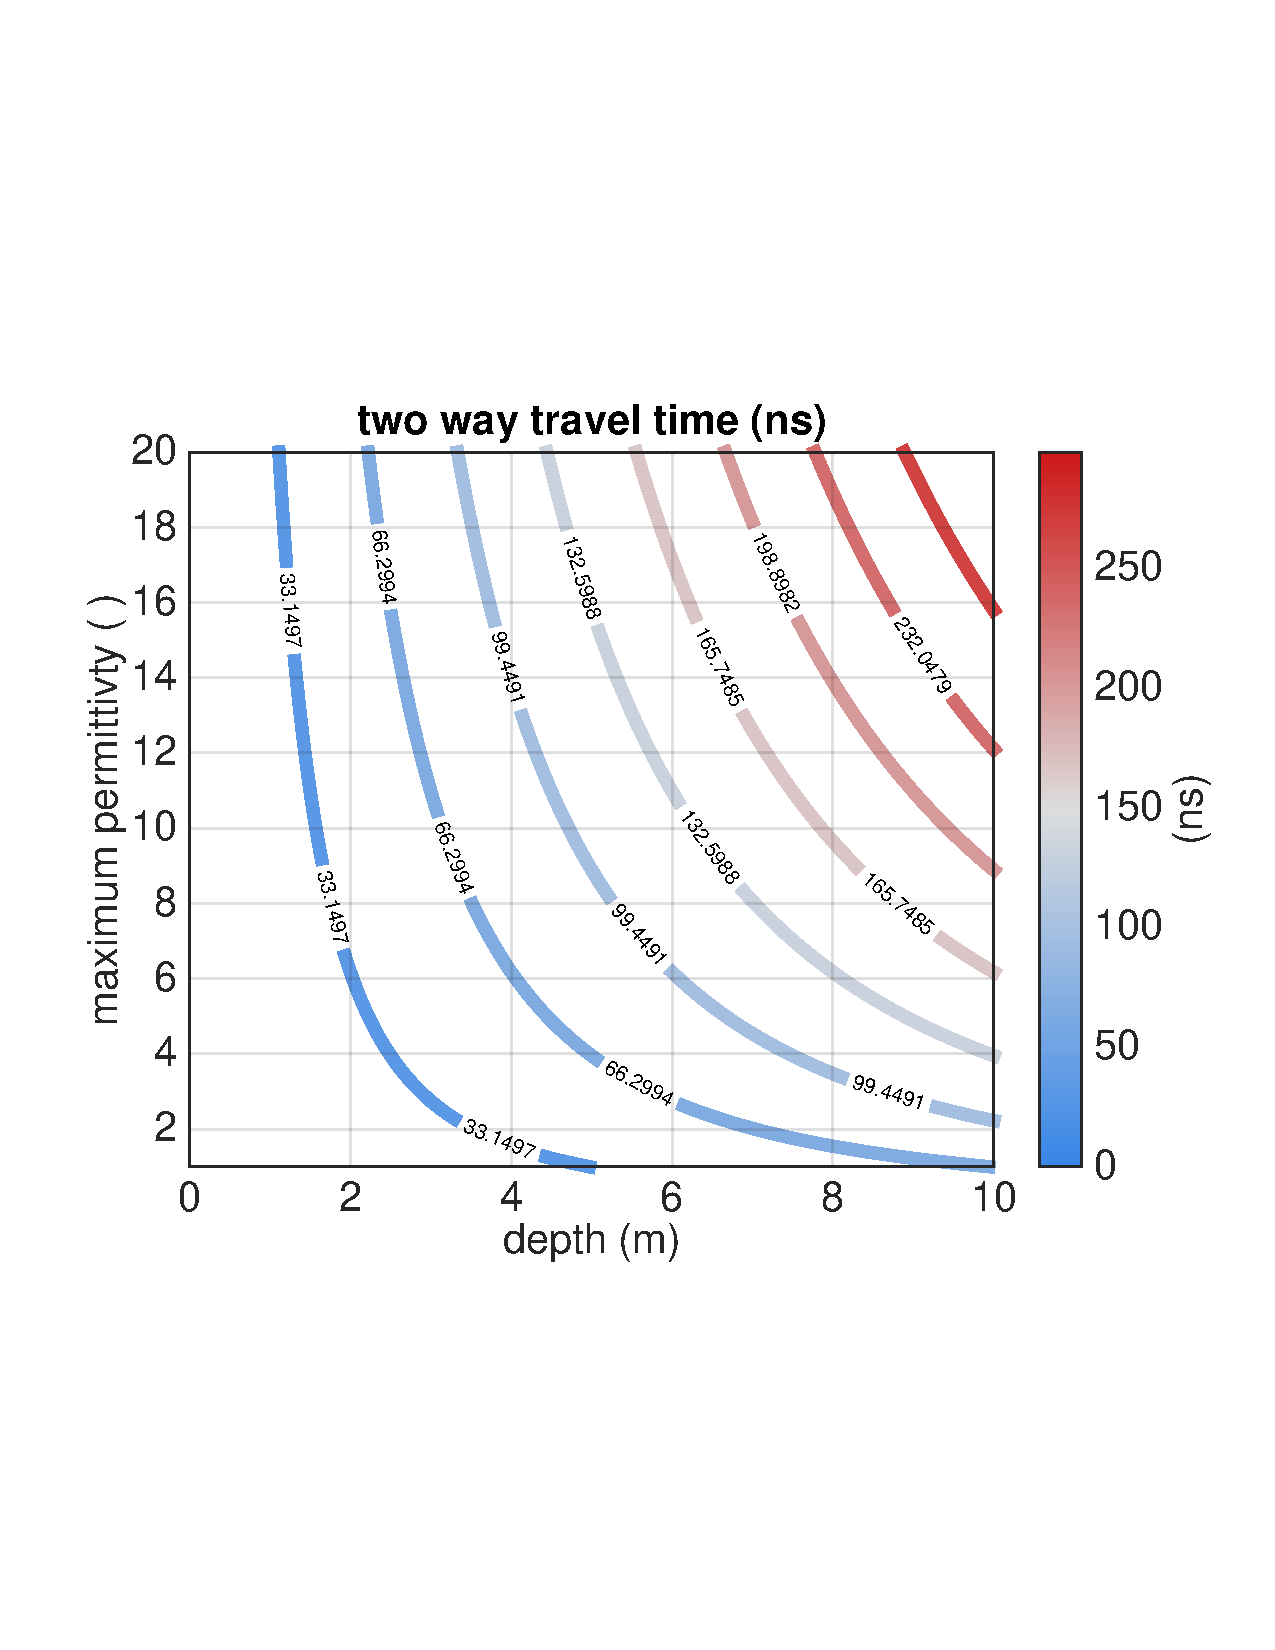
\includegraphics[trim={20 170 30 180},width=\textwidth]{../pics/two-way-time.pdf}
\caption{Two-way travel time as a function of relative permittivity and depth of investigation.}
\label{fig:two-way-time}
\end{figure}
% ------------------------------------------------------
%
% ------------------------------------------------------
\newpage
\section{Common shot gather depth of investigation}
%
%
\begin{figure}[!h]
\centering
% left low right up
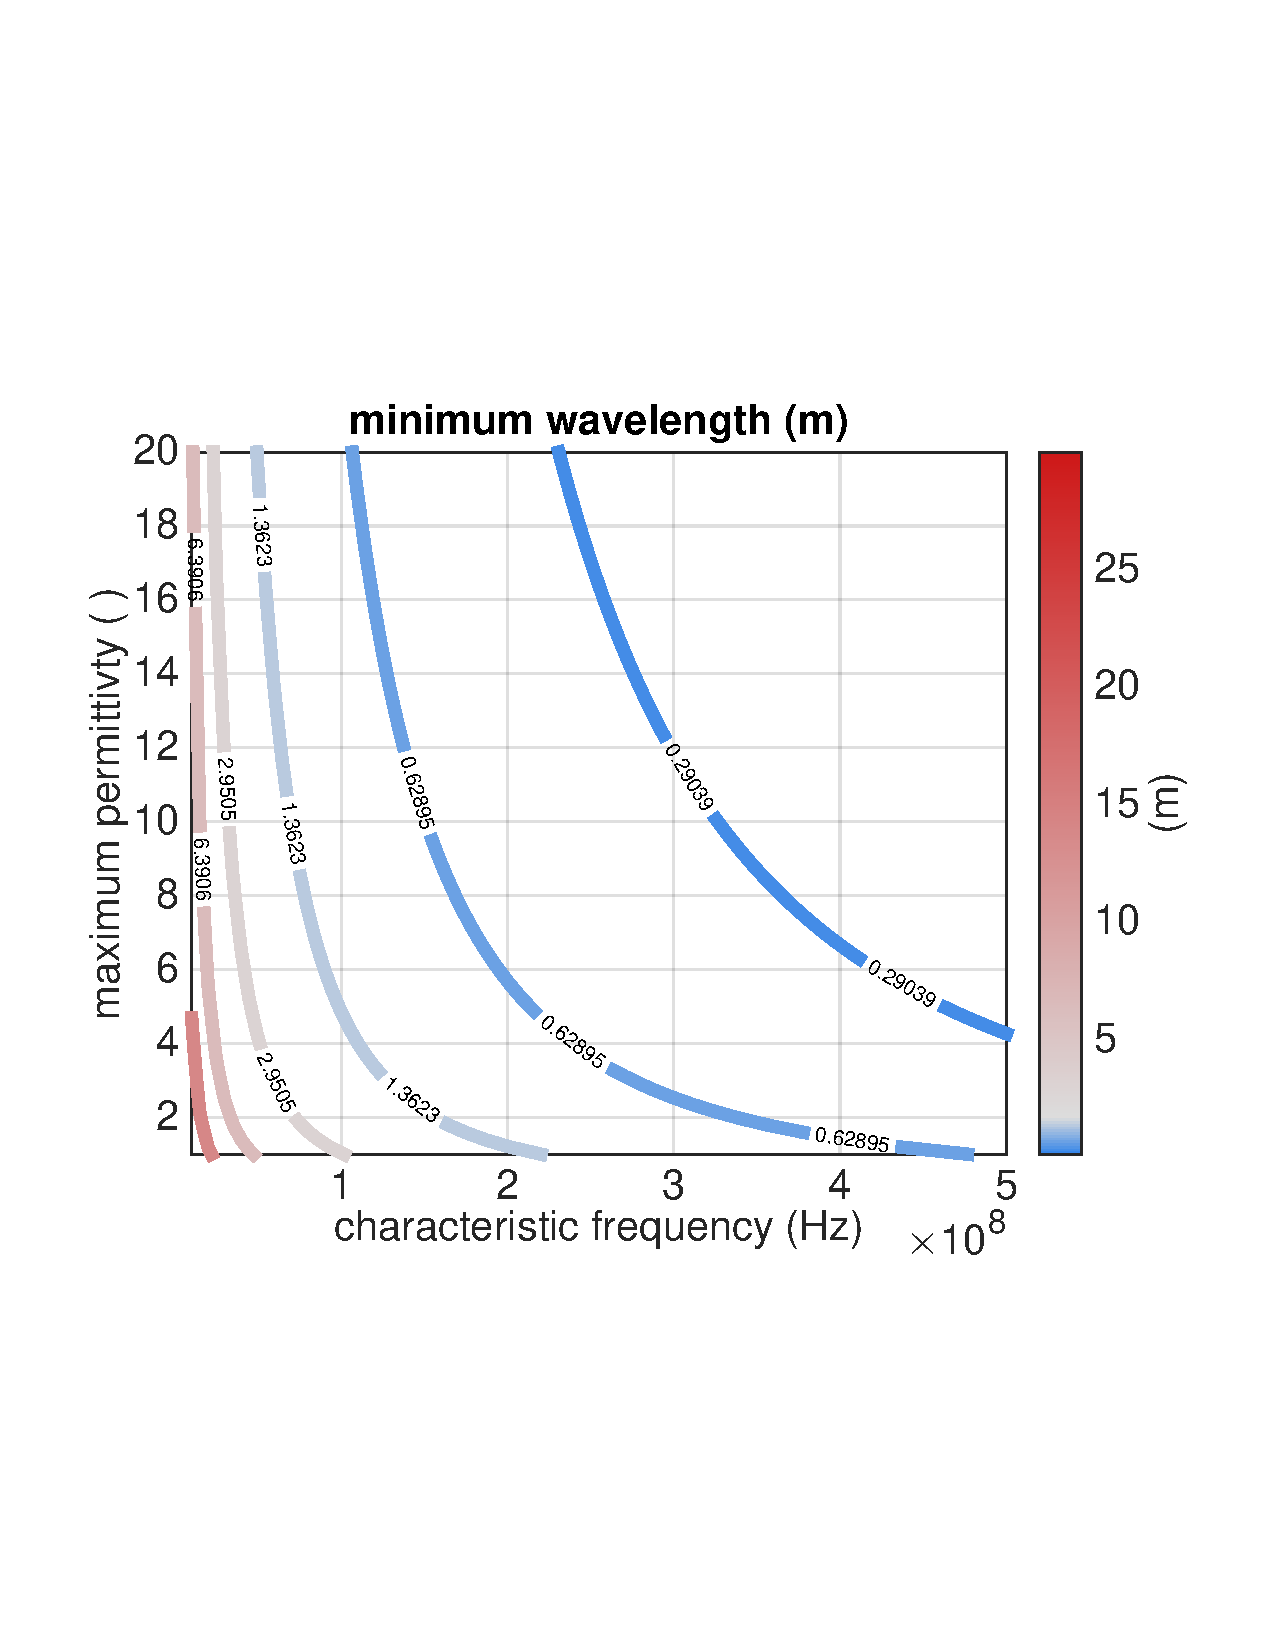
\includegraphics[trim={20 170 30 180},clip,width=0.37\textwidth]{../pics/min-wavelength.pdf}~
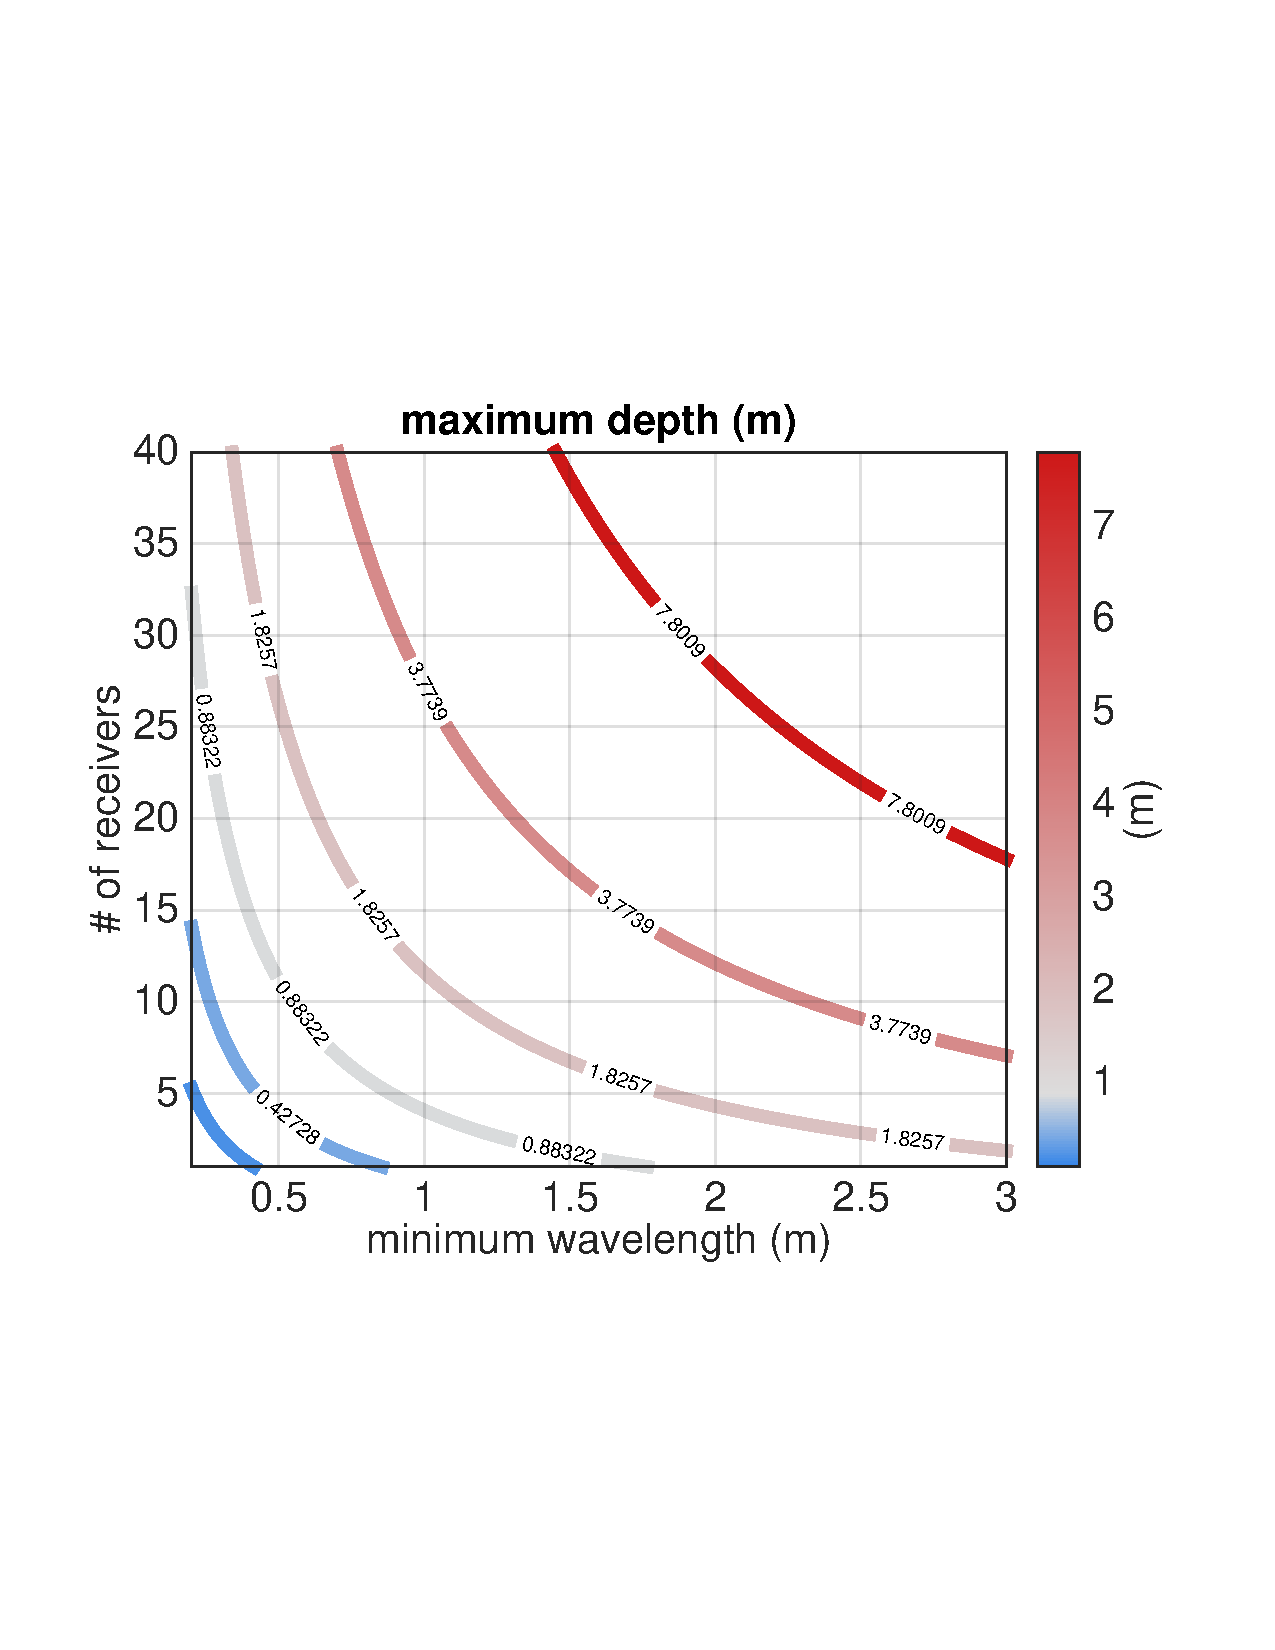
\includegraphics[trim={20 170 30 180},clip,width=0.37\textwidth]{../pics/depth-w.pdf}\\~\\
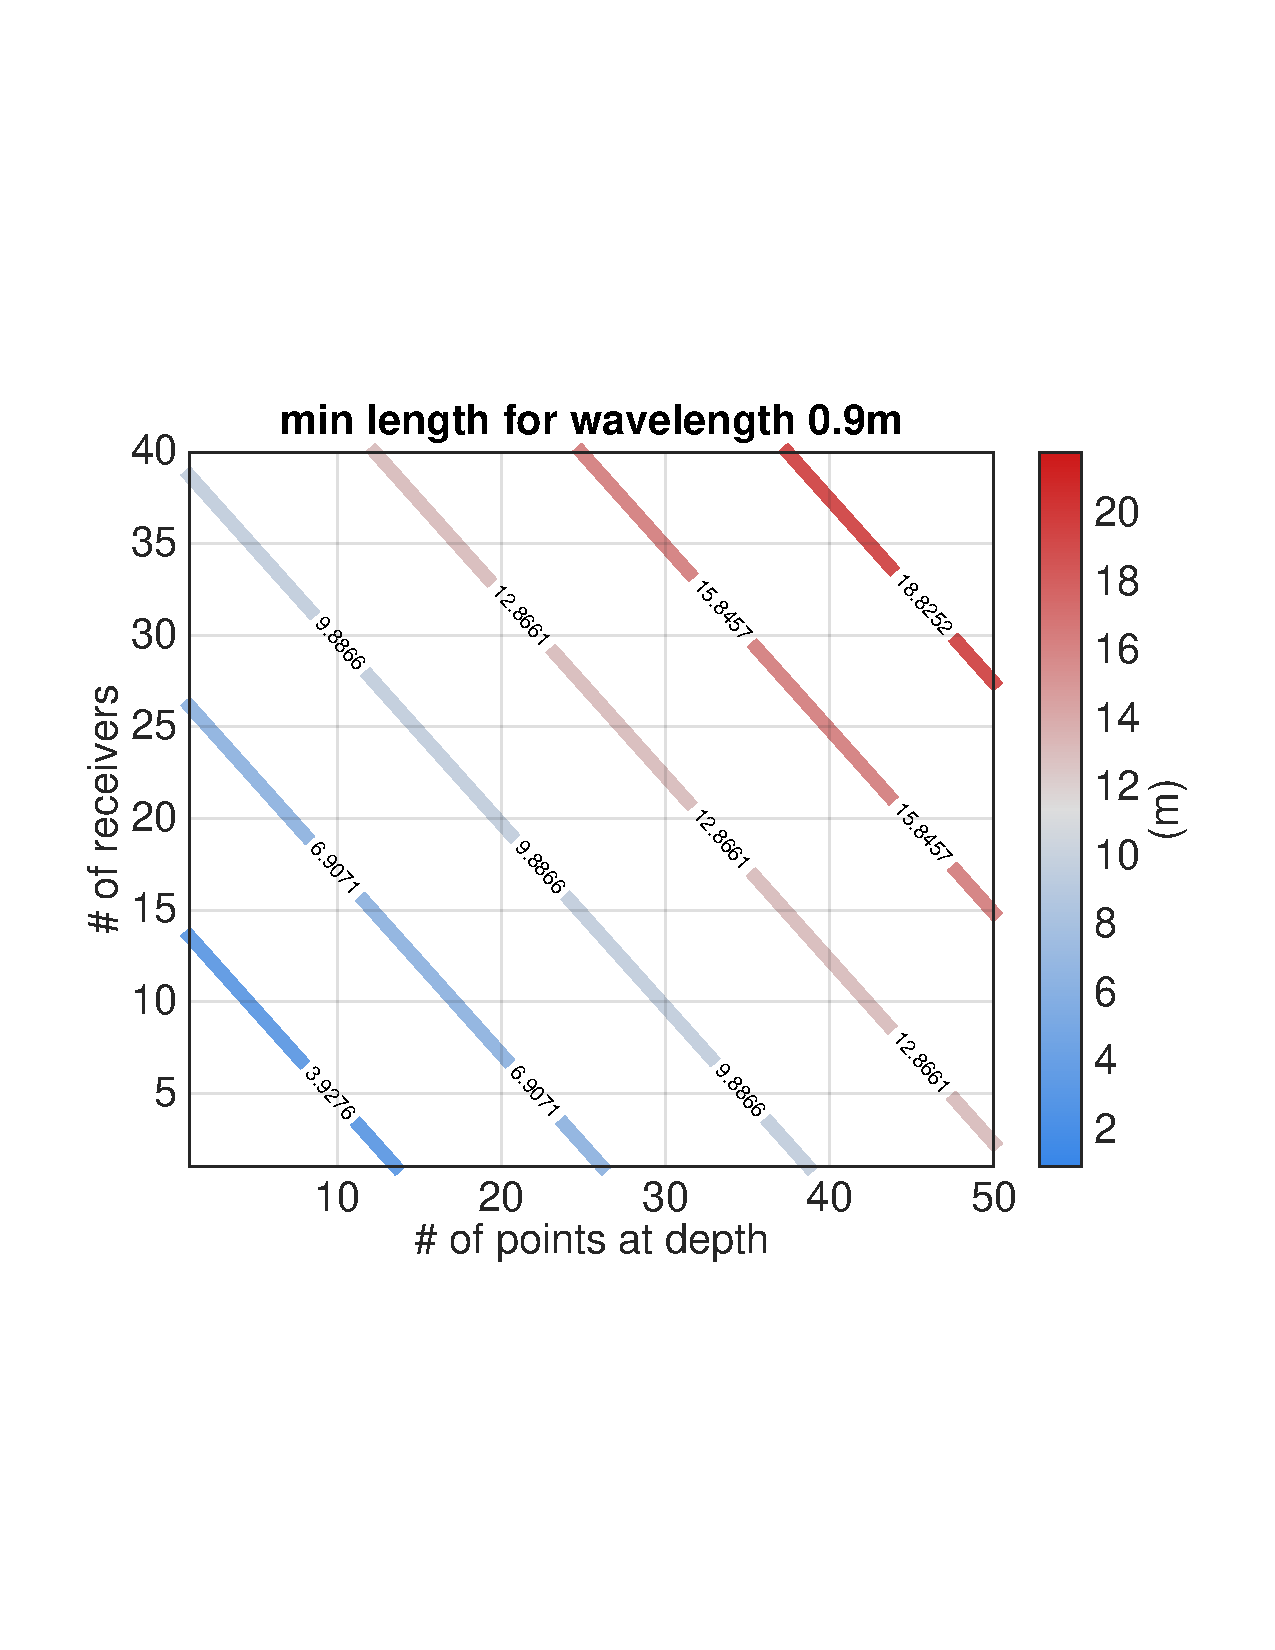
\includegraphics[trim={20 170 30 180},clip,width=0.37\textwidth]{../pics/min-length-wavelength-09m-recs.pdf}~
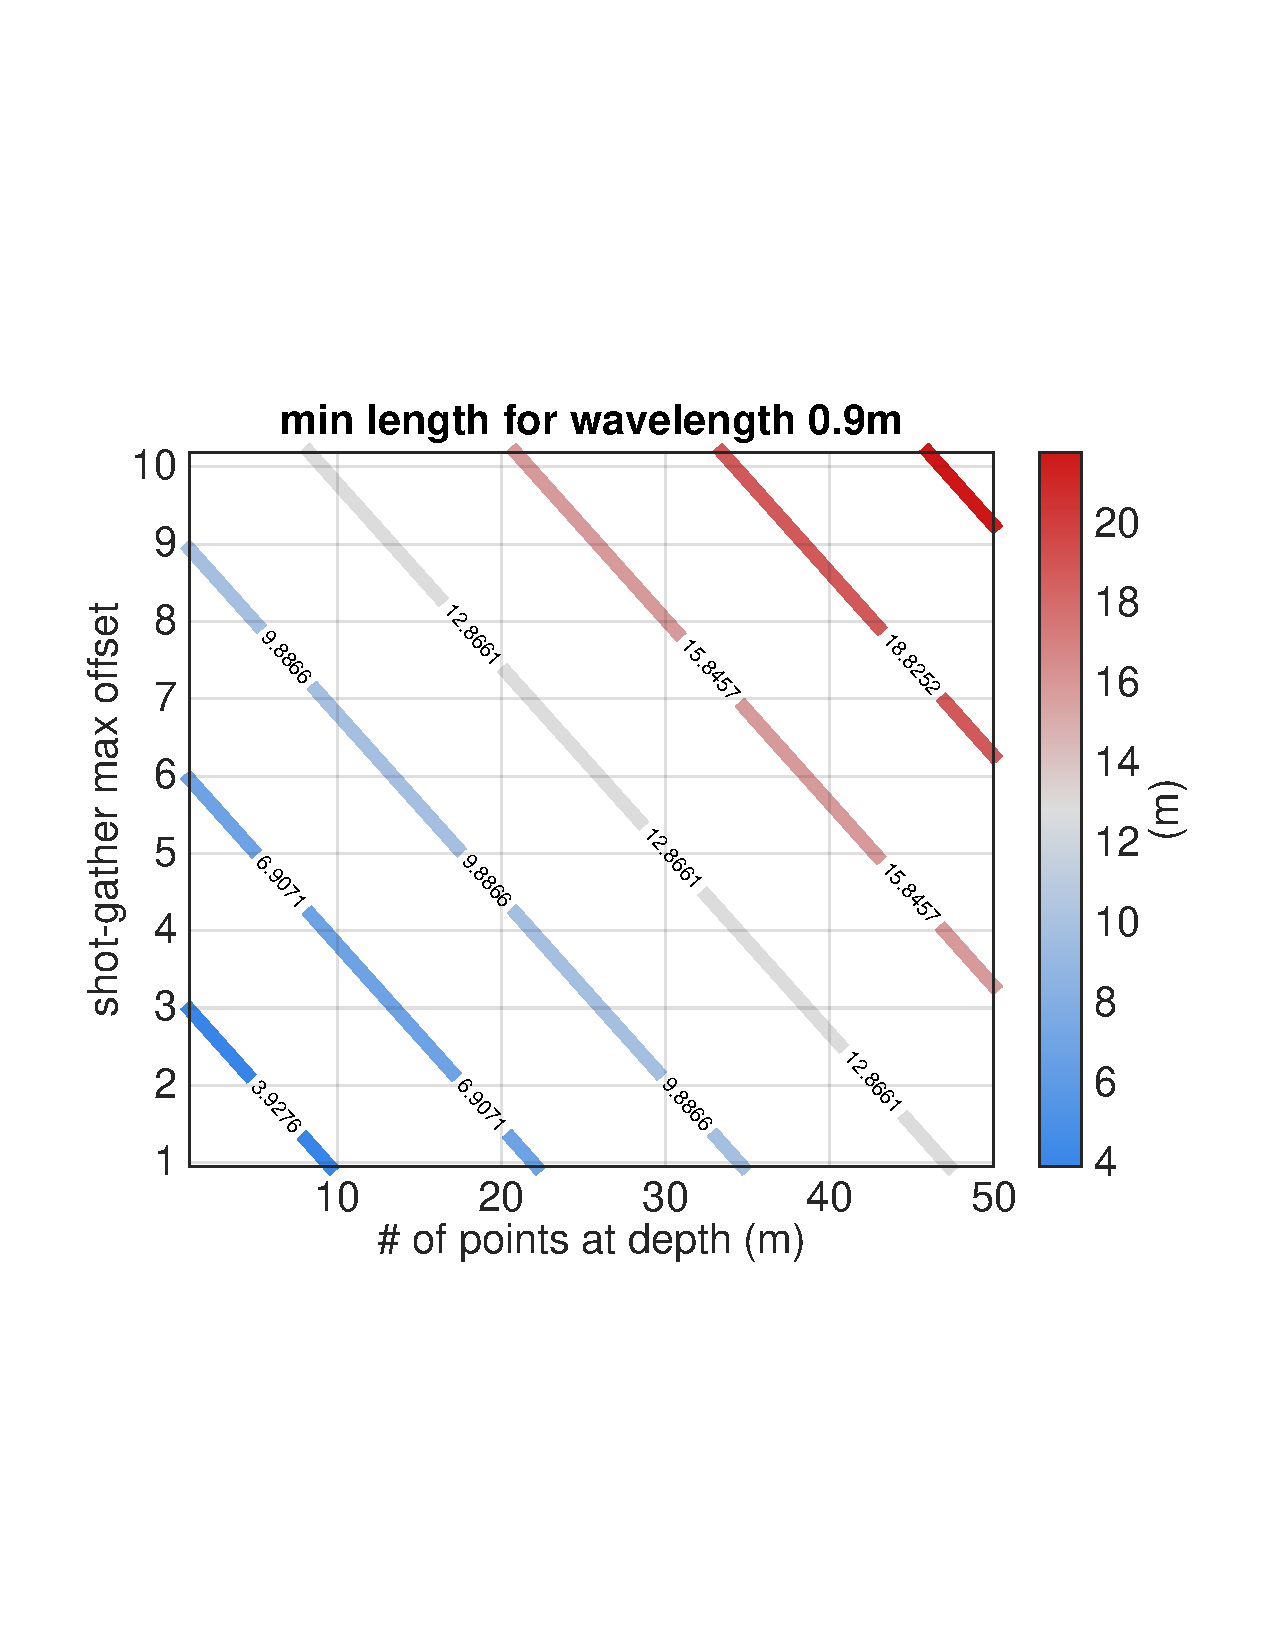
\includegraphics[trim={20 170 30 180},clip,width=0.37\textwidth]{../pics/min-length-wavelength-09m.pdf}
\caption{Plots are read top-bottom, left-right (like reading a book). {\bf b)} and {\bf d)} are specific examples for a fixed frequency and chosen minimum wavelength.}
\label{fig:depth-length}
\end{figure}
%
%
Follow this recipe for determining the depth of investigation and the length of your survey:
\begin{enumerate}
\item See Figure \ref{fig:depth-length}-{\bf a)} and choose the target minimum wavelength as a function of the maximum target permittivity and the characteristic frequency of your system.
\item See \ref{fig:depth-length}-{\bf c)} and choose how deep you want to probe to get the \# of receivers needed for that minimum wavelength and that depth.
\item Run \texttt{w\_depth\_arrays.m} and plot similar Figures \ref{fig:depth-length}-{\bf b)} and {\bf d)} for your chosen minimum wavelength.
\item See Figure \ref{fig:depth-length}-{\bf b)} and determine how many image points at depth you want (this is an empirical computation of the \# of points), and see how many receivers you need for that.
\item Figure \ref{fig:depth-length}-{\bf d)} is one-to-one with Figure \ref{fig:depth-length}-{\bf b)}, so for that \# of receivers you now have a distance in meters for maximum shot-gather offset and the total length of the survey.
\end{enumerate}
% ------------------------------------------------------
%
% ------------------------------------------------------
\newpage
\section{Explanation}
Let $c$ be the speed of light in vacuum and $f_o$ be the characteristic frequency of your GPR system,
\begin{equation}
\begin{aligned}
v&=\frac{c}{\sqrt{\varepsilon}},\\
\lambda_o&=\frac{v_{min}}{f_o}=\frac{c}{f_o\sqrt{\varepsilon_{max}}},
\end{aligned}
\end{equation}
where $\lambda_o$ is the minimum target wavelength. 
\subsection{Two-way traveltime}
For the two-way travel time we have,
\begin{equation}
\begin{aligned}
t&=\frac{z}{2\cdot v}=\frac{z\sqrt{\varepsilon}}{2\cdot c},
\end{aligned}
\end{equation}
where $t$ is two-way travel time and $z$ is depth of investigation with a constant velocity $v$.
\subsection{Depth of investigation and length of common source survey}
Let $n_r$ be the \# of receivers and $n_i$ the \# of illuminated points at depth $z$, where $z$ denotes the maximum depth of sensitivity for the given array. Empirically,
\begin{equation}
\begin{aligned}
2z=x_{sr} &= \Delta sr + (n_r - 1)\Delta r,\\
x &=  x_{sr} + (n_i - 1)\Delta r,
\end{aligned}
\end{equation}
where $x_{sr}$ is the maximum length between source and receiver of a common source gather, and $x$ is the total length of the survey. Our linear array assumes to have distance between source and first receiver $\Delta sr=\lambda_o$, receiver-receiver spacing $\Delta r=\lambda_o/4$, and source-source spacing $\Delta r$.
% ------------------------------------------------------
%
% ------------------------------------------------------
\section{Assumptions}
\begin{itemize}
\item Plane wave
\item Homogeneous velocity model
\item No intrinsic or geometric attenuation
\item No dispersion
\end{itemize}
%
%
\iffalse
\begin{figure}[!h]
\centering
% left low right up
\includegraphics[width=\textwidth]{pics/pics/crop/pdfs/aw-adc-Ew-Edc.png}
\caption{Normalized objective functions history over iterations for the low {\bf a)} and high {\bf c)} conductivity scenarios. Update weights history over iterations for the low {\bf b)} and high {\bf d)} conductivity scenarios}
\label{fig:aw-adc-Ew-Edc}
\end{figure}
\fi
%
%
\end{document}
